% Graphic for TeX using PGF
% Title: D:\Dokumente\GitHub\Bachelorarbeit\Arbeitstagebuch\src\28.06.2017-IRSwTProblem-classdiagram.dia
% Creator: Dia v0.97.2
% CreationDate: Wed Jun 28 15:54:18 2017
% For: Timo Bergerbusch
% \usepackage{tikz}
% The following commands are not supported in PSTricks at present
% We define them conditionally, so when they are implemented,
% this pgf file will use them.
\ifx\du\undefined
  \newlength{\du}
\fi
\setlength{\du}{15\unitlength}
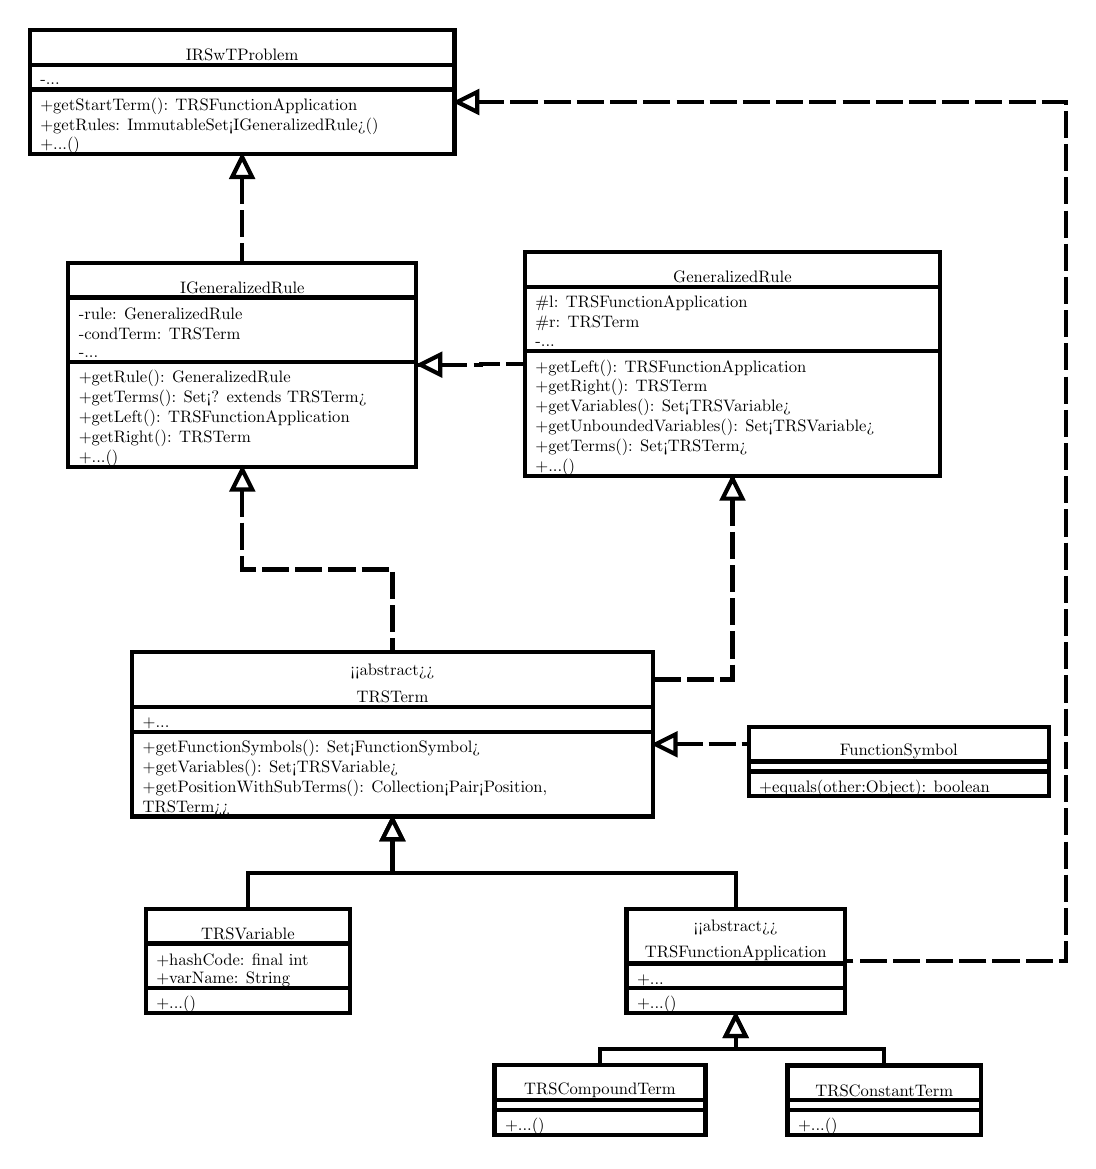
\begin{tikzpicture}[scale=0.6, every node/.style={scale=0.6}]
\pgftransformxscale{1.000000}
\pgftransformyscale{-1.000000}
\definecolor{dialinecolor}{rgb}{0.000000, 0.000000, 0.000000}
\pgfsetstrokecolor{dialinecolor}
\definecolor{dialinecolor}{rgb}{1.000000, 1.000000, 1.000000}
\pgfsetfillcolor{dialinecolor}
\pgfsetlinewidth{0.100000\du}
\pgfsetdash{}{0pt}
\definecolor{dialinecolor}{rgb}{1.000000, 1.000000, 1.000000}
\pgfsetfillcolor{dialinecolor}
\fill (-0.009799\du,1.761248\du)--(-0.009799\du,3.161248\du)--(17.045201\du,3.161248\du)--(17.045201\du,1.761248\du)--cycle;
\definecolor{dialinecolor}{rgb}{0.000000, 0.000000, 0.000000}
\pgfsetstrokecolor{dialinecolor}
\draw (-0.009799\du,1.761248\du)--(-0.009799\du,3.161248\du)--(17.045201\du,3.161248\du)--(17.045201\du,1.761248\du)--cycle;
% setfont left to latex
\definecolor{dialinecolor}{rgb}{0.000000, 0.000000, 0.000000}
\pgfsetstrokecolor{dialinecolor}
\node at (8.517701\du,2.761248\du){IRSwTProblem};
\definecolor{dialinecolor}{rgb}{1.000000, 1.000000, 1.000000}
\pgfsetfillcolor{dialinecolor}
\fill (-0.009799\du,3.161248\du)--(-0.009799\du,4.161248\du)--(17.045201\du,4.161248\du)--(17.045201\du,3.161248\du)--cycle;
\definecolor{dialinecolor}{rgb}{0.000000, 0.000000, 0.000000}
\pgfsetstrokecolor{dialinecolor}
\draw (-0.009799\du,3.161248\du)--(-0.009799\du,4.161248\du)--(17.045201\du,4.161248\du)--(17.045201\du,3.161248\du)--cycle;
% setfont left to latex
\definecolor{dialinecolor}{rgb}{0.000000, 0.000000, 0.000000}
\pgfsetstrokecolor{dialinecolor}
\node[anchor=west] at (0.140201\du,3.821248\du){-...};
\definecolor{dialinecolor}{rgb}{1.000000, 1.000000, 1.000000}
\pgfsetfillcolor{dialinecolor}
\fill (-0.009799\du,4.161248\du)--(-0.009799\du,6.761248\du)--(17.045201\du,6.761248\du)--(17.045201\du,4.161248\du)--cycle;
\definecolor{dialinecolor}{rgb}{0.000000, 0.000000, 0.000000}
\pgfsetstrokecolor{dialinecolor}
\draw (-0.009799\du,4.161248\du)--(-0.009799\du,6.761248\du)--(17.045201\du,6.761248\du)--(17.045201\du,4.161248\du)--cycle;
% setfont left to latex
\definecolor{dialinecolor}{rgb}{0.000000, 0.000000, 0.000000}
\pgfsetstrokecolor{dialinecolor}
\node[anchor=west] at (0.140201\du,4.821248\du){+getStartTerm(): TRSFunctionApplication};
% setfont left to latex
\definecolor{dialinecolor}{rgb}{0.000000, 0.000000, 0.000000}
\pgfsetstrokecolor{dialinecolor}
\node[anchor=west] at (0.140201\du,5.621248\du){+getRules: ImmutableSet<IGeneralizedRule>()};
% setfont left to latex
\definecolor{dialinecolor}{rgb}{0.000000, 0.000000, 0.000000}
\pgfsetstrokecolor{dialinecolor}
\node[anchor=west] at (0.140201\du,6.421248\du){+...()};
\pgfsetlinewidth{0.100000\du}
\pgfsetdash{}{0pt}
\definecolor{dialinecolor}{rgb}{1.000000, 1.000000, 1.000000}
\pgfsetfillcolor{dialinecolor}
\fill (1.536510\du,11.109500\du)--(1.536510\du,12.509500\du)--(15.511510\du,12.509500\du)--(15.511510\du,11.109500\du)--cycle;
\definecolor{dialinecolor}{rgb}{0.000000, 0.000000, 0.000000}
\pgfsetstrokecolor{dialinecolor}
\draw (1.536510\du,11.109500\du)--(1.536510\du,12.509500\du)--(15.511510\du,12.509500\du)--(15.511510\du,11.109500\du)--cycle;
% setfont left to latex
\definecolor{dialinecolor}{rgb}{0.000000, 0.000000, 0.000000}
\pgfsetstrokecolor{dialinecolor}
\node at (8.524010\du,12.109500\du){IGeneralizedRule};
\definecolor{dialinecolor}{rgb}{1.000000, 1.000000, 1.000000}
\pgfsetfillcolor{dialinecolor}
\fill (1.536510\du,12.509500\du)--(1.536510\du,15.109500\du)--(15.511510\du,15.109500\du)--(15.511510\du,12.509500\du)--cycle;
\definecolor{dialinecolor}{rgb}{0.000000, 0.000000, 0.000000}
\pgfsetstrokecolor{dialinecolor}
\draw (1.536510\du,12.509500\du)--(1.536510\du,15.109500\du)--(15.511510\du,15.109500\du)--(15.511510\du,12.509500\du)--cycle;
% setfont left to latex
\definecolor{dialinecolor}{rgb}{0.000000, 0.000000, 0.000000}
\pgfsetstrokecolor{dialinecolor}
\node[anchor=west] at (1.686510\du,13.169500\du){-rule: GeneralizedRule};
% setfont left to latex
\definecolor{dialinecolor}{rgb}{0.000000, 0.000000, 0.000000}
\pgfsetstrokecolor{dialinecolor}
\node[anchor=west] at (1.686510\du,13.969500\du){-condTerm: TRSTerm};
% setfont left to latex
\definecolor{dialinecolor}{rgb}{0.000000, 0.000000, 0.000000}
\pgfsetstrokecolor{dialinecolor}
\node[anchor=west] at (1.686510\du,14.769500\du){-...};
\definecolor{dialinecolor}{rgb}{1.000000, 1.000000, 1.000000}
\pgfsetfillcolor{dialinecolor}
\fill (1.536510\du,15.109500\du)--(1.536510\du,19.309500\du)--(15.511510\du,19.309500\du)--(15.511510\du,15.109500\du)--cycle;
\definecolor{dialinecolor}{rgb}{0.000000, 0.000000, 0.000000}
\pgfsetstrokecolor{dialinecolor}
\draw (1.536510\du,15.109500\du)--(1.536510\du,19.309500\du)--(15.511510\du,19.309500\du)--(15.511510\du,15.109500\du)--cycle;
% setfont left to latex
\definecolor{dialinecolor}{rgb}{0.000000, 0.000000, 0.000000}
\pgfsetstrokecolor{dialinecolor}
\node[anchor=west] at (1.686510\du,15.769500\du){+getRule(): GeneralizedRule};
% setfont left to latex
\definecolor{dialinecolor}{rgb}{0.000000, 0.000000, 0.000000}
\pgfsetstrokecolor{dialinecolor}
\node[anchor=west] at (1.686510\du,16.569500\du){+getTerms(): Set<? extends TRSTerm>};
% setfont left to latex
\definecolor{dialinecolor}{rgb}{0.000000, 0.000000, 0.000000}
\pgfsetstrokecolor{dialinecolor}
\node[anchor=west] at (1.686510\du,17.369500\du){+getLeft(): TRSFunctionApplication};
% setfont left to latex
\definecolor{dialinecolor}{rgb}{0.000000, 0.000000, 0.000000}
\pgfsetstrokecolor{dialinecolor}
\node[anchor=west] at (1.686510\du,18.169500\du){+getRight(): TRSTerm};
% setfont left to latex
\definecolor{dialinecolor}{rgb}{0.000000, 0.000000, 0.000000}
\pgfsetstrokecolor{dialinecolor}
\node[anchor=west] at (1.686510\du,18.969500\du){+...()};
\pgfsetlinewidth{0.100000\du}
\pgfsetdash{}{0pt}
\definecolor{dialinecolor}{rgb}{1.000000, 1.000000, 1.000000}
\pgfsetfillcolor{dialinecolor}
\fill (19.869400\du,10.675900\du)--(19.869400\du,12.075900\du)--(36.539400\du,12.075900\du)--(36.539400\du,10.675900\du)--cycle;
\definecolor{dialinecolor}{rgb}{0.000000, 0.000000, 0.000000}
\pgfsetstrokecolor{dialinecolor}
\draw (19.869400\du,10.675900\du)--(19.869400\du,12.075900\du)--(36.539400\du,12.075900\du)--(36.539400\du,10.675900\du)--cycle;
% setfont left to latex
\definecolor{dialinecolor}{rgb}{0.000000, 0.000000, 0.000000}
\pgfsetstrokecolor{dialinecolor}
\node at (28.204400\du,11.675900\du){GeneralizedRule};
\definecolor{dialinecolor}{rgb}{1.000000, 1.000000, 1.000000}
\pgfsetfillcolor{dialinecolor}
\fill (19.869400\du,12.075900\du)--(19.869400\du,14.675900\du)--(36.539400\du,14.675900\du)--(36.539400\du,12.075900\du)--cycle;
\definecolor{dialinecolor}{rgb}{0.000000, 0.000000, 0.000000}
\pgfsetstrokecolor{dialinecolor}
\draw (19.869400\du,12.075900\du)--(19.869400\du,14.675900\du)--(36.539400\du,14.675900\du)--(36.539400\du,12.075900\du)--cycle;
% setfont left to latex
\definecolor{dialinecolor}{rgb}{0.000000, 0.000000, 0.000000}
\pgfsetstrokecolor{dialinecolor}
\node[anchor=west] at (20.019400\du,12.735900\du){\#l: TRSFunctionApplication};
% setfont left to latex
\definecolor{dialinecolor}{rgb}{0.000000, 0.000000, 0.000000}
\pgfsetstrokecolor{dialinecolor}
\node[anchor=west] at (20.019400\du,13.535900\du){\#r: TRSTerm};
% setfont left to latex
\definecolor{dialinecolor}{rgb}{0.000000, 0.000000, 0.000000}
\pgfsetstrokecolor{dialinecolor}
\node[anchor=west] at (20.019400\du,14.335900\du){-...};
\definecolor{dialinecolor}{rgb}{1.000000, 1.000000, 1.000000}
\pgfsetfillcolor{dialinecolor}
\fill (19.869400\du,14.675900\du)--(19.869400\du,19.675900\du)--(36.539400\du,19.675900\du)--(36.539400\du,14.675900\du)--cycle;
\definecolor{dialinecolor}{rgb}{0.000000, 0.000000, 0.000000}
\pgfsetstrokecolor{dialinecolor}
\draw (19.869400\du,14.675900\du)--(19.869400\du,19.675900\du)--(36.539400\du,19.675900\du)--(36.539400\du,14.675900\du)--cycle;
% setfont left to latex
\definecolor{dialinecolor}{rgb}{0.000000, 0.000000, 0.000000}
\pgfsetstrokecolor{dialinecolor}
\node[anchor=west] at (20.019400\du,15.335900\du){+getLeft(): TRSFunctionApplication};
% setfont left to latex
\definecolor{dialinecolor}{rgb}{0.000000, 0.000000, 0.000000}
\pgfsetstrokecolor{dialinecolor}
\node[anchor=west] at (20.019400\du,16.135900\du){+getRight(): TRSTerm};
% setfont left to latex
\definecolor{dialinecolor}{rgb}{0.000000, 0.000000, 0.000000}
\pgfsetstrokecolor{dialinecolor}
\node[anchor=west] at (20.019400\du,16.935900\du){+getVariables(): Set<TRSVariable>};
% setfont left to latex
\definecolor{dialinecolor}{rgb}{0.000000, 0.000000, 0.000000}
\pgfsetstrokecolor{dialinecolor}
\node[anchor=west] at (20.019400\du,17.735900\du){+getUnboundedVariables(): Set<TRSVariable>};
% setfont left to latex
\definecolor{dialinecolor}{rgb}{0.000000, 0.000000, 0.000000}
\pgfsetstrokecolor{dialinecolor}
\node[anchor=west] at (20.019400\du,18.535900\du){+getTerms(): Set<TRSTerm>};
% setfont left to latex
\definecolor{dialinecolor}{rgb}{0.000000, 0.000000, 0.000000}
\pgfsetstrokecolor{dialinecolor}
\node[anchor=west] at (20.019400\du,19.335900\du){+...()};
\pgfsetlinewidth{0.100000\du}
\pgfsetdash{}{0pt}
\definecolor{dialinecolor}{rgb}{1.000000, 1.000000, 1.000000}
\pgfsetfillcolor{dialinecolor}
\fill (4.100000\du,26.750000\du)--(4.100000\du,28.950000\du)--(25.005000\du,28.950000\du)--(25.005000\du,26.750000\du)--cycle;
\definecolor{dialinecolor}{rgb}{0.000000, 0.000000, 0.000000}
\pgfsetstrokecolor{dialinecolor}
\draw (4.100000\du,26.750000\du)--(4.100000\du,28.950000\du)--(25.005000\du,28.950000\du)--(25.005000\du,26.750000\du)--cycle;
% setfont left to latex
\definecolor{dialinecolor}{rgb}{0.000000, 0.000000, 0.000000}
\pgfsetstrokecolor{dialinecolor}
\node at (14.552500\du,27.510000\du){<<abstract>>};
% setfont left to latex
\definecolor{dialinecolor}{rgb}{0.000000, 0.000000, 0.000000}
\pgfsetstrokecolor{dialinecolor}
\node at (14.552500\du,28.550000\du){TRSTerm};
\definecolor{dialinecolor}{rgb}{1.000000, 1.000000, 1.000000}
\pgfsetfillcolor{dialinecolor}
\fill (4.100000\du,28.950000\du)--(4.100000\du,29.950000\du)--(25.005000\du,29.950000\du)--(25.005000\du,28.950000\du)--cycle;
\definecolor{dialinecolor}{rgb}{0.000000, 0.000000, 0.000000}
\pgfsetstrokecolor{dialinecolor}
\draw (4.100000\du,28.950000\du)--(4.100000\du,29.950000\du)--(25.005000\du,29.950000\du)--(25.005000\du,28.950000\du)--cycle;
% setfont left to latex
\definecolor{dialinecolor}{rgb}{0.000000, 0.000000, 0.000000}
\pgfsetstrokecolor{dialinecolor}
\node[anchor=west] at (4.250000\du,29.610000\du){+...};
\definecolor{dialinecolor}{rgb}{1.000000, 1.000000, 1.000000}
\pgfsetfillcolor{dialinecolor}
\fill (4.100000\du,29.950000\du)--(4.100000\du,33.350000\du)--(25.005000\du,33.350000\du)--(25.005000\du,29.950000\du)--cycle;
\definecolor{dialinecolor}{rgb}{0.000000, 0.000000, 0.000000}
\pgfsetstrokecolor{dialinecolor}
\draw (4.100000\du,29.950000\du)--(4.100000\du,33.350000\du)--(25.005000\du,33.350000\du)--(25.005000\du,29.950000\du)--cycle;
% setfont left to latex
\definecolor{dialinecolor}{rgb}{0.000000, 0.000000, 0.000000}
\pgfsetstrokecolor{dialinecolor}
\node[anchor=west] at (4.250000\du,30.610000\du){+getFunctionSymbols(): Set<FunctionSymbol>};
% setfont left to latex
\definecolor{dialinecolor}{rgb}{0.000000, 0.000000, 0.000000}
\pgfsetstrokecolor{dialinecolor}
\node[anchor=west] at (4.250000\du,31.410000\du){+getVariables(): Set<TRSVariable>};
% setfont left to latex
\definecolor{dialinecolor}{rgb}{0.000000, 0.000000, 0.000000}
\pgfsetstrokecolor{dialinecolor}
\node[anchor=west] at (4.250000\du,32.210000\du){+getPositionWithSubTerms(): Collection<Pair<Position,};
\definecolor{dialinecolor}{rgb}{0.000000, 0.000000, 0.000000}
\pgfsetstrokecolor{dialinecolor}
\node[anchor=west] at (4.250000\du,33.010000\du){                          TRSTerm>>};
\pgfsetlinewidth{0.100000\du}
\pgfsetdash{{1.000000\du}{1.000000\du}}{0\du}
\pgfsetdash{{0.400000\du}{0.400000\du}}{0\du}
\pgfsetmiterjoin
\pgfsetbuttcap
{
\definecolor{dialinecolor}{rgb}{0.000000, 0.000000, 0.000000}
\pgfsetfillcolor{dialinecolor}
% was here!!!
\definecolor{dialinecolor}{rgb}{0.000000, 0.000000, 0.000000}
\pgfsetstrokecolor{dialinecolor}
\draw (8.517701\du,6.761248\du)--(8.517701\du,9.335374\du)--(8.524010\du,9.335374\du)--(8.524010\du,11.109500\du);
}
\definecolor{dialinecolor}{rgb}{0.000000, 0.000000, 0.000000}
\pgfsetstrokecolor{dialinecolor}
\draw (8.517701\du,7.673052\du)--(8.517701\du,9.335374\du)--(8.524010\du,9.335374\du)--(8.524010\du,11.109500\du);
\pgfsetmiterjoin
\definecolor{dialinecolor}{rgb}{1.000000, 1.000000, 1.000000}
\pgfsetfillcolor{dialinecolor}
\fill (8.917701\du,7.673052\du)--(8.517701\du,6.873052\du)--(8.117701\du,7.673052\du)--cycle;
\pgfsetlinewidth{0.100000\du}
\pgfsetdash{}{0pt}
\pgfsetmiterjoin
\definecolor{dialinecolor}{rgb}{0.000000, 0.000000, 0.000000}
\pgfsetstrokecolor{dialinecolor}
\draw (8.917701\du,7.673052\du)--(8.517701\du,6.873052\du)--(8.117701\du,7.673052\du)--cycle;
% setfont left to latex
\pgfsetlinewidth{0.100000\du}
\pgfsetdash{{0.400000\du}{0.400000\du}}{0\du}
\pgfsetdash{{0.400000\du}{0.400000\du}}{0\du}
\pgfsetmiterjoin
\pgfsetbuttcap
{
\definecolor{dialinecolor}{rgb}{0.000000, 0.000000, 0.000000}
\pgfsetfillcolor{dialinecolor}
% was here!!!
\definecolor{dialinecolor}{rgb}{0.000000, 0.000000, 0.000000}
\pgfsetstrokecolor{dialinecolor}
\draw (15.561940\du,15.209500\du)--(18.115670\du,15.209500\du)--(18.115670\du,15.175900\du)--(19.869400\du,15.175900\du);
}
\definecolor{dialinecolor}{rgb}{0.000000, 0.000000, 0.000000}
\pgfsetstrokecolor{dialinecolor}
\draw (16.473743\du,15.209500\du)--(18.115670\du,15.209500\du)--(18.115670\du,15.175900\du)--(19.869400\du,15.175900\du);
\pgfsetmiterjoin
\definecolor{dialinecolor}{rgb}{1.000000, 1.000000, 1.000000}
\pgfsetfillcolor{dialinecolor}
\fill (16.473743\du,14.809500\du)--(15.673743\du,15.209500\du)--(16.473743\du,15.609500\du)--cycle;
\pgfsetlinewidth{0.100000\du}
\pgfsetdash{}{0pt}
\pgfsetmiterjoin
\definecolor{dialinecolor}{rgb}{0.000000, 0.000000, 0.000000}
\pgfsetstrokecolor{dialinecolor}
\draw (16.473743\du,14.809500\du)--(15.673743\du,15.209500\du)--(16.473743\du,15.609500\du)--cycle;
% setfont left to latex
\pgfsetlinewidth{0.100000\du}
\pgfsetdash{{0.400000\du}{0.400000\du}}{0\du}
\pgfsetdash{{0.400000\du}{0.400000\du}}{0\du}
\pgfsetmiterjoin
\pgfsetbuttcap
{
\definecolor{dialinecolor}{rgb}{0.000000, 0.000000, 0.000000}
\pgfsetfillcolor{dialinecolor}
% was here!!!
\definecolor{dialinecolor}{rgb}{0.000000, 0.000000, 0.000000}
\pgfsetstrokecolor{dialinecolor}
\draw (8.524010\du,19.309500\du)--(8.524010\du,23.429750\du)--(14.552500\du,23.429750\du)--(14.552500\du,26.750000\du);
}
\definecolor{dialinecolor}{rgb}{0.000000, 0.000000, 0.000000}
\pgfsetstrokecolor{dialinecolor}
\draw (8.524010\du,20.221303\du)--(8.524010\du,23.429750\du)--(14.552500\du,23.429750\du)--(14.552500\du,26.750000\du);
\pgfsetmiterjoin
\definecolor{dialinecolor}{rgb}{1.000000, 1.000000, 1.000000}
\pgfsetfillcolor{dialinecolor}
\fill (8.924010\du,20.221303\du)--(8.524010\du,19.421303\du)--(8.124010\du,20.221303\du)--cycle;
\pgfsetlinewidth{0.100000\du}
\pgfsetdash{}{0pt}
\pgfsetmiterjoin
\definecolor{dialinecolor}{rgb}{0.000000, 0.000000, 0.000000}
\pgfsetstrokecolor{dialinecolor}
\draw (8.924010\du,20.221303\du)--(8.524010\du,19.421303\du)--(8.124010\du,20.221303\du)--cycle;
% setfont left to latex
\pgfsetlinewidth{0.100000\du}
\pgfsetdash{{0.400000\du}{0.400000\du}}{0\du}
\pgfsetdash{{0.400000\du}{0.400000\du}}{0\du}
\pgfsetmiterjoin
\pgfsetbuttcap
{
\definecolor{dialinecolor}{rgb}{0.000000, 0.000000, 0.000000}
\pgfsetfillcolor{dialinecolor}
% was here!!!
\definecolor{dialinecolor}{rgb}{0.000000, 0.000000, 0.000000}
\pgfsetstrokecolor{dialinecolor}
\draw (28.204400\du,19.675900\du)--(28.204400\du,27.850000\du)--(25.005000\du,27.850000\du);
}
\definecolor{dialinecolor}{rgb}{0.000000, 0.000000, 0.000000}
\pgfsetstrokecolor{dialinecolor}
\draw (28.204400\du,20.587703\du)--(28.204400\du,27.850000\du)--(25.005000\du,27.850000\du);
\pgfsetmiterjoin
\definecolor{dialinecolor}{rgb}{1.000000, 1.000000, 1.000000}
\pgfsetfillcolor{dialinecolor}
\fill (28.604400\du,20.587703\du)--(28.204400\du,19.787703\du)--(27.804400\du,20.587703\du)--cycle;
\pgfsetlinewidth{0.100000\du}
\pgfsetdash{}{0pt}
\pgfsetmiterjoin
\definecolor{dialinecolor}{rgb}{0.000000, 0.000000, 0.000000}
\pgfsetstrokecolor{dialinecolor}
\draw (28.604400\du,20.587703\du)--(28.204400\du,19.787703\du)--(27.804400\du,20.587703\du)--cycle;
% setfont left to latex
\pgfsetlinewidth{0.100000\du}
\pgfsetdash{}{0pt}
\definecolor{dialinecolor}{rgb}{1.000000, 1.000000, 1.000000}
\pgfsetfillcolor{dialinecolor}
\fill (28.855631\du,29.740728\du)--(28.855631\du,31.140728\du)--(40.905631\du,31.140728\du)--(40.905631\du,29.740728\du)--cycle;
\definecolor{dialinecolor}{rgb}{0.000000, 0.000000, 0.000000}
\pgfsetstrokecolor{dialinecolor}
\draw (28.855631\du,29.740728\du)--(28.855631\du,31.140728\du)--(40.905631\du,31.140728\du)--(40.905631\du,29.740728\du)--cycle;
% setfont left to latex
\definecolor{dialinecolor}{rgb}{0.000000, 0.000000, 0.000000}
\pgfsetstrokecolor{dialinecolor}
\node at (34.880631\du,30.740728\du){FunctionSymbol};
\definecolor{dialinecolor}{rgb}{1.000000, 1.000000, 1.000000}
\pgfsetfillcolor{dialinecolor}
\fill (28.855631\du,31.140728\du)--(28.855631\du,31.540728\du)--(40.905631\du,31.540728\du)--(40.905631\du,31.140728\du)--cycle;
\definecolor{dialinecolor}{rgb}{0.000000, 0.000000, 0.000000}
\pgfsetstrokecolor{dialinecolor}
\draw (28.855631\du,31.140728\du)--(28.855631\du,31.540728\du)--(40.905631\du,31.540728\du)--(40.905631\du,31.140728\du)--cycle;
\definecolor{dialinecolor}{rgb}{1.000000, 1.000000, 1.000000}
\pgfsetfillcolor{dialinecolor}
\fill (28.855631\du,31.540728\du)--(28.855631\du,32.540728\du)--(40.905631\du,32.540728\du)--(40.905631\du,31.540728\du)--cycle;
\definecolor{dialinecolor}{rgb}{0.000000, 0.000000, 0.000000}
\pgfsetstrokecolor{dialinecolor}
\draw (28.855631\du,31.540728\du)--(28.855631\du,32.540728\du)--(40.905631\du,32.540728\du)--(40.905631\du,31.540728\du)--cycle;
% setfont left to latex
\definecolor{dialinecolor}{rgb}{0.000000, 0.000000, 0.000000}
\pgfsetstrokecolor{dialinecolor}
\node[anchor=west] at (29.005631\du,32.200728\du){+equals(other:Object): boolean};
\pgfsetlinewidth{0.100000\du}
\pgfsetdash{{0.400000\du}{0.400000\du}}{0\du}
\pgfsetdash{{0.400000\du}{0.400000\du}}{0\du}
\pgfsetmiterjoin
\pgfsetbuttcap
{
\definecolor{dialinecolor}{rgb}{0.000000, 0.000000, 0.000000}
\pgfsetfillcolor{dialinecolor}
% was here!!!
\definecolor{dialinecolor}{rgb}{0.000000, 0.000000, 0.000000}
\pgfsetstrokecolor{dialinecolor}
\draw (25.005000\du,30.450000\du)--(27.330315\du,30.450000\du)--(27.330315\du,30.440728\du)--(28.855631\du,30.440728\du);
}
\definecolor{dialinecolor}{rgb}{0.000000, 0.000000, 0.000000}
\pgfsetstrokecolor{dialinecolor}
\draw (25.916803\du,30.450000\du)--(27.330315\du,30.450000\du)--(27.330315\du,30.440728\du)--(28.855631\du,30.440728\du);
\pgfsetmiterjoin
\definecolor{dialinecolor}{rgb}{1.000000, 1.000000, 1.000000}
\pgfsetfillcolor{dialinecolor}
\fill (25.916803\du,30.050000\du)--(25.116803\du,30.450000\du)--(25.916803\du,30.850000\du)--cycle;
\pgfsetlinewidth{0.100000\du}
\pgfsetdash{}{0pt}
\pgfsetmiterjoin
\definecolor{dialinecolor}{rgb}{0.000000, 0.000000, 0.000000}
\pgfsetstrokecolor{dialinecolor}
\draw (25.916803\du,30.050000\du)--(25.116803\du,30.450000\du)--(25.916803\du,30.850000\du)--cycle;
% setfont left to latex
\pgfsetlinewidth{0.100000\du}
\pgfsetdash{}{0pt}
\definecolor{dialinecolor}{rgb}{1.000000, 1.000000, 1.000000}
\pgfsetfillcolor{dialinecolor}
\fill (23.950000\du,37.050000\du)--(23.950000\du,39.250000\du)--(32.717500\du,39.250000\du)--(32.717500\du,37.050000\du)--cycle;
\definecolor{dialinecolor}{rgb}{0.000000, 0.000000, 0.000000}
\pgfsetstrokecolor{dialinecolor}
\draw (23.950000\du,37.050000\du)--(23.950000\du,39.250000\du)--(32.717500\du,39.250000\du)--(32.717500\du,37.050000\du)--cycle;
% setfont left to latex
\definecolor{dialinecolor}{rgb}{0.000000, 0.000000, 0.000000}
\pgfsetstrokecolor{dialinecolor}
\node at (28.333750\du,37.810000\du){<<abstract>>};
% setfont left to latex
\definecolor{dialinecolor}{rgb}{0.000000, 0.000000, 0.000000}
\pgfsetstrokecolor{dialinecolor}
\node at (28.333750\du,38.850000\du){TRSFunctionApplication};
\definecolor{dialinecolor}{rgb}{1.000000, 1.000000, 1.000000}
\pgfsetfillcolor{dialinecolor}
\fill (23.950000\du,39.250000\du)--(23.950000\du,40.250000\du)--(32.717500\du,40.250000\du)--(32.717500\du,39.250000\du)--cycle;
\definecolor{dialinecolor}{rgb}{0.000000, 0.000000, 0.000000}
\pgfsetstrokecolor{dialinecolor}
\draw (23.950000\du,39.250000\du)--(23.950000\du,40.250000\du)--(32.717500\du,40.250000\du)--(32.717500\du,39.250000\du)--cycle;
% setfont left to latex
\definecolor{dialinecolor}{rgb}{0.000000, 0.000000, 0.000000}
\pgfsetstrokecolor{dialinecolor}
\node[anchor=west] at (24.100000\du,39.910000\du){+...};
\definecolor{dialinecolor}{rgb}{1.000000, 1.000000, 1.000000}
\pgfsetfillcolor{dialinecolor}
\fill (23.950000\du,40.250000\du)--(23.950000\du,41.250000\du)--(32.717500\du,41.250000\du)--(32.717500\du,40.250000\du)--cycle;
\definecolor{dialinecolor}{rgb}{0.000000, 0.000000, 0.000000}
\pgfsetstrokecolor{dialinecolor}
\draw (23.950000\du,40.250000\du)--(23.950000\du,41.250000\du)--(32.717500\du,41.250000\du)--(32.717500\du,40.250000\du)--cycle;
% setfont left to latex
\definecolor{dialinecolor}{rgb}{0.000000, 0.000000, 0.000000}
\pgfsetstrokecolor{dialinecolor}
\node[anchor=west] at (24.100000\du,40.910000\du){+...()};
\pgfsetlinewidth{0.100000\du}
\pgfsetdash{}{0pt}
\pgfsetmiterjoin
\pgfsetbuttcap
{
\definecolor{dialinecolor}{rgb}{0.000000, 0.000000, 0.000000}
\pgfsetfillcolor{dialinecolor}
% was here!!!
\definecolor{dialinecolor}{rgb}{0.000000, 0.000000, 0.000000}
\pgfsetstrokecolor{dialinecolor}
\draw (14.552500\du,33.350000\du)--(14.552500\du,35.600000\du)--(28.333750\du,35.600000\du)--(28.333750\du,37.050000\du);
}
\definecolor{dialinecolor}{rgb}{0.000000, 0.000000, 0.000000}
\pgfsetstrokecolor{dialinecolor}
\draw (14.552500\du,34.261803\du)--(14.552500\du,35.600000\du)--(28.333750\du,35.600000\du)--(28.333750\du,37.050000\du);
\pgfsetmiterjoin
\definecolor{dialinecolor}{rgb}{1.000000, 1.000000, 1.000000}
\pgfsetfillcolor{dialinecolor}
\fill (14.952500\du,34.261803\du)--(14.552500\du,33.461803\du)--(14.152500\du,34.261803\du)--cycle;
\pgfsetlinewidth{0.100000\du}
\pgfsetdash{}{0pt}
\pgfsetmiterjoin
\definecolor{dialinecolor}{rgb}{0.000000, 0.000000, 0.000000}
\pgfsetstrokecolor{dialinecolor}
\draw (14.952500\du,34.261803\du)--(14.552500\du,33.461803\du)--(14.152500\du,34.261803\du)--cycle;
% setfont left to latex
\pgfsetlinewidth{0.100000\du}
\pgfsetdash{}{0pt}
\definecolor{dialinecolor}{rgb}{1.000000, 1.000000, 1.000000}
\pgfsetfillcolor{dialinecolor}
\fill (4.650000\du,37.050000\du)--(4.650000\du,38.450000\du)--(12.850000\du,38.450000\du)--(12.850000\du,37.050000\du)--cycle;
\definecolor{dialinecolor}{rgb}{0.000000, 0.000000, 0.000000}
\pgfsetstrokecolor{dialinecolor}
\draw (4.650000\du,37.050000\du)--(4.650000\du,38.450000\du)--(12.850000\du,38.450000\du)--(12.850000\du,37.050000\du)--cycle;
% setfont left to latex
\definecolor{dialinecolor}{rgb}{0.000000, 0.000000, 0.000000}
\pgfsetstrokecolor{dialinecolor}
\node at (8.750000\du,38.050000\du){TRSVariable};
\definecolor{dialinecolor}{rgb}{1.000000, 1.000000, 1.000000}
\pgfsetfillcolor{dialinecolor}
\fill (4.650000\du,38.450000\du)--(4.650000\du,40.250000\du)--(12.850000\du,40.250000\du)--(12.850000\du,38.450000\du)--cycle;
\definecolor{dialinecolor}{rgb}{0.000000, 0.000000, 0.000000}
\pgfsetstrokecolor{dialinecolor}
\draw (4.650000\du,38.450000\du)--(4.650000\du,40.250000\du)--(12.850000\du,40.250000\du)--(12.850000\du,38.450000\du)--cycle;
% setfont left to latex
\definecolor{dialinecolor}{rgb}{0.000000, 0.000000, 0.000000}
\pgfsetstrokecolor{dialinecolor}
\node[anchor=west] at (4.800000\du,39.110000\du){+hashCode: final int};
% setfont left to latex
\definecolor{dialinecolor}{rgb}{0.000000, 0.000000, 0.000000}
\pgfsetstrokecolor{dialinecolor}
\node[anchor=west] at (4.800000\du,39.910000\du){+varName: String};
\definecolor{dialinecolor}{rgb}{1.000000, 1.000000, 1.000000}
\pgfsetfillcolor{dialinecolor}
\fill (4.650000\du,40.250000\du)--(4.650000\du,41.250000\du)--(12.850000\du,41.250000\du)--(12.850000\du,40.250000\du)--cycle;
\definecolor{dialinecolor}{rgb}{0.000000, 0.000000, 0.000000}
\pgfsetstrokecolor{dialinecolor}
\draw (4.650000\du,40.250000\du)--(4.650000\du,41.250000\du)--(12.850000\du,41.250000\du)--(12.850000\du,40.250000\du)--cycle;
% setfont left to latex
\definecolor{dialinecolor}{rgb}{0.000000, 0.000000, 0.000000}
\pgfsetstrokecolor{dialinecolor}
\node[anchor=west] at (4.800000\du,40.910000\du){+...()};
\pgfsetlinewidth{0.100000\du}
\pgfsetdash{}{0pt}
\pgfsetmiterjoin
\pgfsetbuttcap
{
\definecolor{dialinecolor}{rgb}{0.000000, 0.000000, 0.000000}
\pgfsetfillcolor{dialinecolor}
% was here!!!
\definecolor{dialinecolor}{rgb}{0.000000, 0.000000, 0.000000}
\pgfsetstrokecolor{dialinecolor}
\draw (14.552500\du,33.350000\du)--(14.552500\du,35.600000\du)--(8.750000\du,35.600000\du)--(8.750000\du,37.050000\du);
}
\definecolor{dialinecolor}{rgb}{0.000000, 0.000000, 0.000000}
\pgfsetstrokecolor{dialinecolor}
\draw (14.552500\du,34.261803\du)--(14.552500\du,35.600000\du)--(8.750000\du,35.600000\du)--(8.750000\du,37.050000\du);
\pgfsetmiterjoin
\definecolor{dialinecolor}{rgb}{1.000000, 1.000000, 1.000000}
\pgfsetfillcolor{dialinecolor}
\fill (14.952500\du,34.261803\du)--(14.552500\du,33.461803\du)--(14.152500\du,34.261803\du)--cycle;
\pgfsetlinewidth{0.100000\du}
\pgfsetdash{}{0pt}
\pgfsetmiterjoin
\definecolor{dialinecolor}{rgb}{0.000000, 0.000000, 0.000000}
\pgfsetstrokecolor{dialinecolor}
\draw (14.952500\du,34.261803\du)--(14.552500\du,33.461803\du)--(14.152500\du,34.261803\du)--cycle;
% setfont left to latex
\pgfsetlinewidth{0.100000\du}
\pgfsetdash{}{0pt}
\definecolor{dialinecolor}{rgb}{1.000000, 1.000000, 1.000000}
\pgfsetfillcolor{dialinecolor}
\fill (18.649779\du,43.342276\du)--(18.649779\du,44.742276\du)--(27.119779\du,44.742276\du)--(27.119779\du,43.342276\du)--cycle;
\definecolor{dialinecolor}{rgb}{0.000000, 0.000000, 0.000000}
\pgfsetstrokecolor{dialinecolor}
\draw (18.649779\du,43.342276\du)--(18.649779\du,44.742276\du)--(27.119779\du,44.742276\du)--(27.119779\du,43.342276\du)--cycle;
% setfont left to latex
\definecolor{dialinecolor}{rgb}{0.000000, 0.000000, 0.000000}
\pgfsetstrokecolor{dialinecolor}
\node at (22.884779\du,44.342276\du){TRSCompoundTerm};
\definecolor{dialinecolor}{rgb}{1.000000, 1.000000, 1.000000}
\pgfsetfillcolor{dialinecolor}
\fill (18.649779\du,44.742276\du)--(18.649779\du,45.142276\du)--(27.119779\du,45.142276\du)--(27.119779\du,44.742276\du)--cycle;
\definecolor{dialinecolor}{rgb}{0.000000, 0.000000, 0.000000}
\pgfsetstrokecolor{dialinecolor}
\draw (18.649779\du,44.742276\du)--(18.649779\du,45.142276\du)--(27.119779\du,45.142276\du)--(27.119779\du,44.742276\du)--cycle;
\definecolor{dialinecolor}{rgb}{1.000000, 1.000000, 1.000000}
\pgfsetfillcolor{dialinecolor}
\fill (18.649779\du,45.142276\du)--(18.649779\du,46.142276\du)--(27.119779\du,46.142276\du)--(27.119779\du,45.142276\du)--cycle;
\definecolor{dialinecolor}{rgb}{0.000000, 0.000000, 0.000000}
\pgfsetstrokecolor{dialinecolor}
\draw (18.649779\du,45.142276\du)--(18.649779\du,46.142276\du)--(27.119779\du,46.142276\du)--(27.119779\du,45.142276\du)--cycle;
% setfont left to latex
\definecolor{dialinecolor}{rgb}{0.000000, 0.000000, 0.000000}
\pgfsetstrokecolor{dialinecolor}
\node[anchor=west] at (18.799779\du,45.802276\du){+...()};
\pgfsetlinewidth{0.100000\du}
\pgfsetdash{}{0pt}
\definecolor{dialinecolor}{rgb}{1.000000, 1.000000, 1.000000}
\pgfsetfillcolor{dialinecolor}
\fill (30.414018\du,43.346801\du)--(30.414018\du,44.746801\du)--(38.179018\du,44.746801\du)--(38.179018\du,43.346801\du)--cycle;
\definecolor{dialinecolor}{rgb}{0.000000, 0.000000, 0.000000}
\pgfsetstrokecolor{dialinecolor}
\draw (30.414018\du,43.346801\du)--(30.414018\du,44.746801\du)--(38.179018\du,44.746801\du)--(38.179018\du,43.346801\du)--cycle;
% setfont left to latex
\definecolor{dialinecolor}{rgb}{0.000000, 0.000000, 0.000000}
\pgfsetstrokecolor{dialinecolor}
\node at (34.296518\du,44.346801\du){TRSConstantTerm};
\definecolor{dialinecolor}{rgb}{1.000000, 1.000000, 1.000000}
\pgfsetfillcolor{dialinecolor}
\fill (30.414018\du,44.746801\du)--(30.414018\du,45.146801\du)--(38.179018\du,45.146801\du)--(38.179018\du,44.746801\du)--cycle;
\definecolor{dialinecolor}{rgb}{0.000000, 0.000000, 0.000000}
\pgfsetstrokecolor{dialinecolor}
\draw (30.414018\du,44.746801\du)--(30.414018\du,45.146801\du)--(38.179018\du,45.146801\du)--(38.179018\du,44.746801\du)--cycle;
\definecolor{dialinecolor}{rgb}{1.000000, 1.000000, 1.000000}
\pgfsetfillcolor{dialinecolor}
\fill (30.414018\du,45.146801\du)--(30.414018\du,46.146801\du)--(38.179018\du,46.146801\du)--(38.179018\du,45.146801\du)--cycle;
\definecolor{dialinecolor}{rgb}{0.000000, 0.000000, 0.000000}
\pgfsetstrokecolor{dialinecolor}
\draw (30.414018\du,45.146801\du)--(30.414018\du,46.146801\du)--(38.179018\du,46.146801\du)--(38.179018\du,45.146801\du)--cycle;
% setfont left to latex
\definecolor{dialinecolor}{rgb}{0.000000, 0.000000, 0.000000}
\pgfsetstrokecolor{dialinecolor}
\node[anchor=west] at (30.564018\du,45.806801\du){+...()};
\pgfsetlinewidth{0.100000\du}
\pgfsetdash{}{0pt}
\pgfsetmiterjoin
\pgfsetbuttcap
{
\definecolor{dialinecolor}{rgb}{0.000000, 0.000000, 0.000000}
\pgfsetfillcolor{dialinecolor}
% was here!!!
\definecolor{dialinecolor}{rgb}{0.000000, 0.000000, 0.000000}
\pgfsetstrokecolor{dialinecolor}
\draw (28.333750\du,41.250000\du)--(28.333750\du,42.696138\du)--(22.884779\du,42.696138\du)--(22.884779\du,43.342276\du);
}
\definecolor{dialinecolor}{rgb}{0.000000, 0.000000, 0.000000}
\pgfsetstrokecolor{dialinecolor}
\draw (28.333750\du,42.161803\du)--(28.333750\du,42.696138\du)--(22.884779\du,42.696138\du)--(22.884779\du,43.342276\du);
\pgfsetmiterjoin
\definecolor{dialinecolor}{rgb}{1.000000, 1.000000, 1.000000}
\pgfsetfillcolor{dialinecolor}
\fill (28.733750\du,42.161803\du)--(28.333750\du,41.361803\du)--(27.933750\du,42.161803\du)--cycle;
\pgfsetlinewidth{0.100000\du}
\pgfsetdash{}{0pt}
\pgfsetmiterjoin
\definecolor{dialinecolor}{rgb}{0.000000, 0.000000, 0.000000}
\pgfsetstrokecolor{dialinecolor}
\draw (28.733750\du,42.161803\du)--(28.333750\du,41.361803\du)--(27.933750\du,42.161803\du)--cycle;
% setfont left to latex
\pgfsetlinewidth{0.100000\du}
\pgfsetdash{}{0pt}
\pgfsetmiterjoin
\pgfsetbuttcap
{
\definecolor{dialinecolor}{rgb}{0.000000, 0.000000, 0.000000}
\pgfsetfillcolor{dialinecolor}
% was here!!!
\definecolor{dialinecolor}{rgb}{0.000000, 0.000000, 0.000000}
\pgfsetstrokecolor{dialinecolor}
\draw (28.333750\du,41.250000\du)--(28.333750\du,42.698401\du)--(34.296518\du,42.698401\du)--(34.296518\du,43.346801\du);
}
\definecolor{dialinecolor}{rgb}{0.000000, 0.000000, 0.000000}
\pgfsetstrokecolor{dialinecolor}
\draw (28.333750\du,42.161803\du)--(28.333750\du,42.698401\du)--(34.296518\du,42.698401\du)--(34.296518\du,43.346801\du);
\pgfsetmiterjoin
\definecolor{dialinecolor}{rgb}{1.000000, 1.000000, 1.000000}
\pgfsetfillcolor{dialinecolor}
\fill (28.733750\du,42.161803\du)--(28.333750\du,41.361803\du)--(27.933750\du,42.161803\du)--cycle;
\pgfsetlinewidth{0.100000\du}
\pgfsetdash{}{0pt}
\pgfsetmiterjoin
\definecolor{dialinecolor}{rgb}{0.000000, 0.000000, 0.000000}
\pgfsetstrokecolor{dialinecolor}
\draw (28.733750\du,42.161803\du)--(28.333750\du,41.361803\du)--(27.933750\du,42.161803\du)--cycle;
% setfont left to latex
\pgfsetlinewidth{0.100000\du}
\pgfsetdash{{0.400000\du}{0.400000\du}}{0\du}
\pgfsetdash{{0.400000\du}{0.400000\du}}{0\du}
\pgfsetmiterjoin
\pgfsetbuttcap
{
\definecolor{dialinecolor}{rgb}{0.000000, 0.000000, 0.000000}
\pgfsetfillcolor{dialinecolor}
% was here!!!
\definecolor{dialinecolor}{rgb}{0.000000, 0.000000, 0.000000}
\pgfsetstrokecolor{dialinecolor}
\draw (17.045201\du,4.661248\du)--(41.597574\du,4.661248\du)--(41.597574\du,39.150000\du)--(32.767303\du,39.150000\du);
}
\definecolor{dialinecolor}{rgb}{0.000000, 0.000000, 0.000000}
\pgfsetstrokecolor{dialinecolor}
\draw (17.957005\du,4.661248\du)--(41.597574\du,4.661248\du)--(41.597574\du,39.150000\du)--(32.767303\du,39.150000\du);
\pgfsetmiterjoin
\definecolor{dialinecolor}{rgb}{1.000000, 1.000000, 1.000000}
\pgfsetfillcolor{dialinecolor}
\fill (17.957005\du,4.261248\du)--(17.157005\du,4.661248\du)--(17.957005\du,5.061248\du)--cycle;
\pgfsetlinewidth{0.100000\du}
\pgfsetdash{}{0pt}
\pgfsetmiterjoin
\definecolor{dialinecolor}{rgb}{0.000000, 0.000000, 0.000000}
\pgfsetstrokecolor{dialinecolor}
\draw (17.957005\du,4.261248\du)--(17.157005\du,4.661248\du)--(17.957005\du,5.061248\du)--cycle;
% setfont left to latex
\end{tikzpicture}
